% Begin the document and set up the style of the document
\documentclass[a4paper]{article}

% Install the required packages for the document 
\usepackage{envmath}
\usepackage{esvect}
\usepackage{graphicx}
\usepackage{gensymb}
\usepackage{tikz}
\usepackage{geometry}
\usepackage{enumitem}
\usepackage{mathtools}
\usepackage{graphicx}
\usepackage{amsmath}
\usepackage{amscd}
\usepackage{amssymb}
\usepackage{amsfonts}
\usepackage{pgf}
\usepackage{tikz}
\usepackage{mathrsfs}
\usepackage{asyalign}
\usepackage{physics}
\usepackage{cite}
\usepackage{url}
\usepackage[tableposition=top]{caption}
\usepackage{ifthen}
\usepackage[utf8]{inputenc}
\usetikzlibrary{arrows}

\begin{document}

\begin{center}
	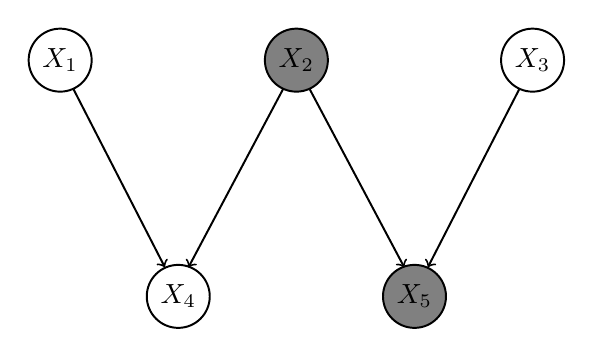
\begin{tikzpicture}

		\draw[line width = 0.25mm] (-3,3) circle (4mm);
		\node at (-3,3) {$X_1$};
		\draw[line width = 0.25mm][fill = gray] (0,3) circle (4mm);
		\node at (0,3) {$X_2$};
		\draw[line width = 0.25mm] (3,3) circle (4mm);
		\node at (3,3) {$X_3$};

		\draw[line width = 0.25mm] (-1.5,0) circle (4mm);
		\node at (-1.5,0) {$X_4$};
		\draw[line width = 0.25mm][fill = gray] (1.5,0) circle (4mm);
		\node at (1.5,0) {$X_5$};

		\draw[line width = 0.25mm][->] (-2.83,2.63) -- (-1.67,0.37);

		\draw[line width = 0.25mm][->] (-0.17,2.63) -- (-1.37,0.37);

		\draw[line width = 0.25mm][->] (0.17,2.63) -- (1.37,0.37);

		\draw[line width = 0.25mm][->] (2.83,2.63) -- (1.67,0.37);

	\end{tikzpicture}
\end{center}

\end{document}
